\section{Decomposition 2: OtherFunctionality1 (M1, P2, UC11)}

\subsection{Module to decompose}
    In this run we decompose OtherFunctionality1.


\subsection{Selected architectural drivers}
    The non-functional drivers for this decomposition are:
    \begin{itemize}
    	\item \emph{M1}: Integrate new sensor or actuator manufacturer
        \item \emph{P2}: Requests to the pluggable data database
    \end{itemize}

    \noindent The related functional drivers are:
    \begin{itemize}
        \item \emph{UC11}: Send pluggable device data (P2) \\
              This use case stores pluggable device data in the pluggable device data storage.
              This could be a sensor reading or an actuator status.
    \end{itemize}

    \paragraph{Rationale}
    We chose M1 as it was one of the remaining quality attributes with high priority.
    M1's focus on easily introducing new types of devices to the system is very important
    because of the fast growing market for IoT and development of applications for IoT.
    Thus, we want to handle this quality attribute before U2 (the other remaining
    attribute with high priority), as we presume that customer organisations
    are more interested in using new devices than the effort it takes for
    infrastructure owners to install the devices. \\
    We also chose P2 because it is strongly related to M1; the whole data flow from
    devices to storage/applications needs to exist before modifications can even be made.
    This combination of M1 and P2 would force us to handle processing and
    storage of data while making the involved components as simple as possible to modify.


\subsection{Architectural design}
    This section describes what needs to be done to satisfy the requirements for
    this decomposition and how involved problems/obstacles are solved.
    % Tactics:
    %     Limit event response? reply within response measure deadlines
    %     Prioritize events
    %     Introduce concurrency
    %     Schedule resources

    % Tactics M1:
    %     reduce size of modules: split module

    \paragraph{M1: Handling new types of pluggable devices}
        The new types of sensor or actuator data should be transmitted, processed and stored,
        and should be made available to applications. The infrastructure managers must be able to initialize the new type of pluggable device
        (UC8 : Initialise a pluggable device), configure access rights for these devices (UC9 : Con-
        figure pluggable device access rights), and view detailed information about the new type
        of pluggable device (UC10 : Consult and configure the topology).

        The developers have to make changes to: component1, component2, datatype X.
        The new type of sensor needs to be able to be initialised so that it can send data.
        Thus, the PluggableDeviceFacade code that initialises devices should be updated for
        each new type of sensor. The PluggableDeviceData datatype should be updated to
        represent the new type of data. In this case, the new type will have to be added
        to the database that contains all different types of sensor data.

    \paragraph{M1: Data conversions}
        The pluggable data processing subsystem should be extended with relevant data conver-
        sions, e.g. converting temperature in degrees Fahrenheit to degrees Celsius.\
        \texttt{The PluggableDeviceDataConverter} is resposible for converting data
         in system, for instance converting temperature in degrees Fahrenheit
         to degrees Celsius. System has to work with relevant data,
         otherwise problem may arise.

    \paragraph{M1: Usage of new data by applications}
        The available applications can be updated to use any new pluggable devices.

        This is possible through the RequestData interface provided by PluggableDeviceDataScheduler.
        The application manager can get device data from the PluggableDeviceDB and return this
        data to applications in the PluggableDeviceData datatype. This datatype can easily be
        updated for new types of pluggable devices.

    \paragraph{M1: Configuration of new device by infrastructure owners}
        Initialisation: IO triggers the initialise() method which has been
        updated for the new pluggable device -> OK\\
        Configure access rights: has absolutely fucking nothing to do with the
        new sensor type -> OK \\
        Consult and configure topology: same as configure access rights

    \paragraph{P2: Scheduling}
        - In normal mode, the database processes incoming requests in a first-in-first-out order.
        - If the system fails to comply to the deadlines specified below, it goes in overload mode: requests
            are handled in the order that returns the system to normal mode the fastest, taking into
            account:
            ∗ the nature of the requests: storing new pluggable data (UC11 : Send pluggable device
            data) has priority over specific lookup queries (e.g. retrieving most recent measurement
            for a few sensors), which in turn have priority over broad queries (e.g. retrieving all sensor
            data for the last month).
            ∗ the priority of an application: requests from applications marked as critical by their sub-
            scribers are processed before non-critical applications.
        - Also a mechanism should be in place to avoid starvation of any type of request.

        dynamic priority scheduling \\
        tactics: schedule resource, prioritize events, also limit event response?\\
        starvation avoidance

    \paragraph{P2: Pluggable data separation}
        The processing of (large amounts of) requests concerning pluggable data has no impact on
        requests concerning other data, e.g. available applications.

        "pluggable data has no impact on other data"
        two databases

    \subsubsection{Alternatives considered}
        \paragraph{Alternatives for solution}
            A discussion of the alternative solutions and why that were not selected.


\subsection{Instantiation and allocation of functionality}
    This section describes the new components which instantiate our solutions described
    in the section above and how components are deployed on physical nodes. \\
    Unless stated otherwise the responsibilities assigned in the first decomposition are unchanged.

    \paragraph{Decomposition}
        Figure \ref{fig:it2-cc_main} shows the components resulting from the
        decomposition in this run.

        \begin{figure}[!h]
        	\centering
            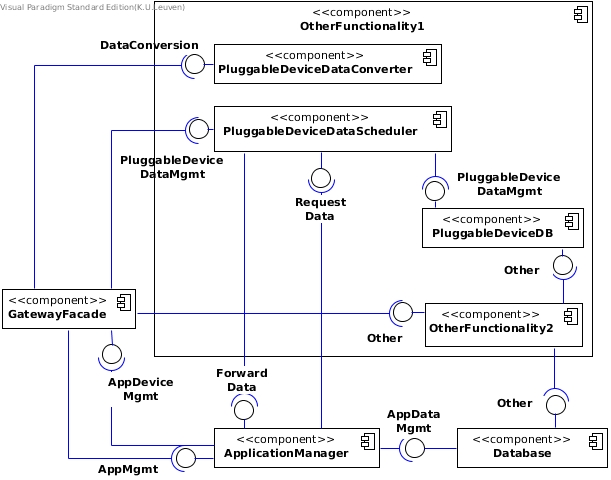
\includegraphics[width=1\textwidth]{component-diagram-2}
        	\caption{Component-and-connector diagram of this decomposition.}
            \label{fig:it2-cc_main}
        \end{figure}

        \noindent The responsibilities of the components are as follows:

    \subparagraph{PluggableDeviceDB}
        store data related to pluggable devices

    \subparagraph{PluggableDeviceDataScheduler}
        scheduling, detect overload mode, store data, forward data

    \subparagraph{PluggableDeviceDataConverter}
        M1: conversion of new type of data of new type of device

    % \paragraph{Behaviour}
        % A SEQUENCE DIAGRAM WOULD BE USEFUL FOR
        % UC11: shows how the gateway checks if devices are initialised
        % UC14: shows how applications can get deactivated

    \paragraph{Deployment}
        Figure \ref{fig:it2-depl_main} shows the allocation of components
        to physical nodes.

        \begin{figure}[!h]
        	\centering
        	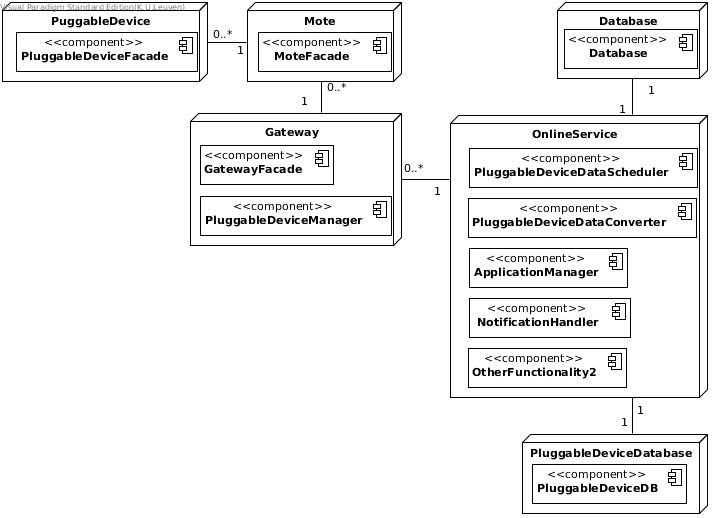
\includegraphics[width=1\textwidth]{deployment-diagram-2}
        	\caption{Deployment diagram of this decomposition.
        	}\label{fig:it2-depl_main}
        \end{figure}


\subsection{Interfaces for child modules}\label{add2-interfaces}
    This section describes the interfaces assigned to the components defined
    in the section above. Per interface, we list its methods by means of its
    syntax. The data types used in these interfaces are defined in the following section. \\

    \noindent Each method shows which (part of a) quality attribute or use case caused
    a need for the method. However, this does not mean that a method is
    only to be used to satisfy that quality  attribute or use case, it could
    be used for other causes not yet mentioned here.

    \noindent The interfaces and methods defined here are to be seen as an
    extension of the interfaces defined in previous sections, unless
    explicitly stated otherwise.

    \subsubsection{GatewayFacade}
        \begin{itemize}
            \item MoteDataMgmt, last defined in section \ref{add1-interfaces}
            \begin{itemize}
                \item \texttt{void sendData(PluggableDeviceData data)}
                \begin{itemize}
                    \item Effect: Sends pluggable device data to the connected mote.
                    \item Created for:
                \end{itemize}
            \end{itemize}

            \item DeviceMgmt, last defined in section \ref{add1-interfaces}
            \begin{itemize}
                \item \texttt{void initialiseDevice(int deviceID, PluggableDeviceSettings settings)}
                \begin{itemize}
                    \item Effect: Initialises a pluggable device for use with the system.
                    \item Created for:
                \end{itemize}
            \end{itemize}

            \item AppDeviceMgmt, last defined in section \ref{add1-interfaces}
            \begin{itemize}
                \item \texttt{void configurePluggableDevice(int deviceID, PluggableDeviceSettings settings)}
                \begin{itemize}
                    \item For: Use case 11 step 3.b
                    \item Effect: Causes certain settings to be set on a pluggable
                          device that the gateway is connected to.
                    \item Created for:
                \end{itemize}
            \end{itemize}
        \end{itemize}

    \subsubsection{MoteFacade}
        \begin{itemize}
            \item PluggableDeviceDataMgmt, last defined in section \ref{add1-interfaces}
            \begin{itemize}
                \item \texttt{void sendData(PluggableDeviceData data)}
                \begin{itemize}
                    \item Effect: Sends pluggable device data to the connected mote.
                    \item Created for:
                \end{itemize}
            \end{itemize}

            \item PluggableDeviceMgmt
            \begin{itemize}
                \item \texttt{void initialise(int deviceID, PluggableDeviceSettings settings)}
                \begin{itemize}
                    \item Effect: Initialises a connected pluggable device according to some settings
                    \item Created for:
                \end{itemize}
            \end{itemize}
        \end{itemize}

    \subsubsection{PluggableDeviceFacade}
        \begin{itemize}
        	\item PluggableDeviceMgmt
        	\begin{itemize}
                \item \texttt{void initialise(PluggableDeviceSettings settings)}
                \begin{itemize}
                    \item Effect: Initialises the pluggable device according to some settings
                    \item Created for:
                \end{itemize}
        	\end{itemize}
        \end{itemize}

    \subsubsection{PluggableDeviceManager}
        \begin{itemize}
        	\item DeviceListMgmt, last defined in section \ref{add1-interfaces}
        	\begin{itemize}
        		\item \texttt{bool isDeviceInitialised(int deviceID)}
        		\begin{itemize}
        			\item Effect: Returns true if the device with id "deviceID" has been initialized.
        			\item Created for:
        		\end{itemize}
        	\end{itemize}
        \end{itemize}

    \subsubsection{PluggableDeviceDataScheduler}
        \begin{itemize}
            \item RequestData
            \begin{itemize}
                \item \texttt{List<PluggableDeviceData> requestData(int applicationID, int deviceID, DateTime from, DateTime to)}
                \begin{itemize}
                    \item Effect: Request data from a specific device in a certain time period
                    \item Created for:
                \end{itemize}
            \end{itemize}

            \item PluggableDeviceDataMgmt
            \begin{itemize}
                \item \texttt{void sendData(PluggableDeviceData data)}
                \begin{itemize}
                    \item Effect: Sends pluggable device data to the scheduler to be processed.
                    \item Created for:
                \end{itemize}
            \end{itemize}
        \end{itemize}

    \subsubsection{PluggableDeviceDB}
        \begin{itemize}
            \item PluggableDeviceDataMgmt
            \begin{itemize}
                \item \texttt{void sendData(PluggableDeviceData data)}
                \begin{itemize}
                    \item Effect: Sends pluggable device data to the DB to be stored.
                    \item Created for:
                \end{itemize}
                \item \texttt{List<PluggableDeviceData> getData(int deviceID, DateTime from, DateTime to)}
                \begin{itemize}
                    \item Effect: Returns data from a specific device in a certain time period.
                    \item Created for:
                \end{itemize}
                \item \texttt{List<int> getApplicationsForDevice(int deviceID)}
                \begin{itemize}
                    \item Effect: Returns a list of applications that can use the device with id "deviceID."
                    \item Created for:
                \end{itemize}
            \end{itemize}
        \end{itemize}


\subsection{Data type definitions}
    This section defines new data types that are used in the interface descriptions above.

    \paragraph{DateTime} Represents an instant in time, typically expressed as a date and time of day.


\subsection{Verify and refine}
    \noindent The selected architectural drivers have been handled completely
    in this decomposition.
    This section describes per component which (parts of) the remaining
    requirements it is responsible for. If requirements are split in
    multiple parts, this is indicated by the addition of a letter
    (or number, depending on the structure of the requirement) after their title.

    \paragraph{ApplicationManager}
        \begin{itemize}
            \item \emph{Av2}: Application failure \\
                   Prevention: a, b \\
                   Detection: a, b, c \\
                   Resolution: a, b, c
           \item \emph{P1}: Large number of users: c
           \item \emph{M2}: Big data analytics on pluggable data and/or application usage data: d, e
           \item \emph{U1}: Application updates: a, b, c, d
           \item \emph{U2}: Easy Installation: e
           \item \emph{UC12}: Perform actuation command
           \item \emph{UC17}: Activate an application: 3, 4
        \end{itemize}

    \paragraph{Database}
        \begin{itemize}
          	\item None
        \end{itemize}

    \paragraph{GatewayFacade}
        \begin{itemize}
            \item \emph{Av1}: Communication between SIoTIP gateway and Online Service \\
                               Resolution: b, c, d
            \item \emph{U2}: Easy Installation: a, c, d
        \end{itemize}

    \paragraph{MoteFacade}
        \begin{itemize}
            \item \emph{U2}: Easy Installation: b, c, d
            \item \emph{UC04}: Install mote: 1, 2
            \item \emph{UC05}: Uninstall mote: 1
            \item \emph{UC06}: Insert a pluggable device into a mote: 2
            \item \emph{UC07}: Remove a pluggable device from its mote: 2
        \end{itemize}

    \paragraph{NotificationHandler}
        \begin{itemize}
            \item \emph{UC16}: Consult notification message: 5
            \item \emph{UC17}: Activate an application: 5, 6
        \end{itemize}

    \paragraph{OtherFunctionality2}
        \begin{itemize}
            \item \emph{Av1}: Communication between SIoTIP gateway and Online Service \\
                               Detection: a, b, c, d
                               Resolution: a
           	\item \emph{P1}: Large number of users: a
            \item \emph{M2}: Big data analytics on pluggable data and/or application usage data: a
            \item \emph{U2}: Easy Installation: e
            \item \emph{UC01}: Register a customer organisation
            \item \emph{UC02}: Register an end-user
            \item \emph{UC03}: Unregister an end user
            \item \emph{UC04}: Install mote: 3
            \item \emph{UC05}: Uninstall mote: 2.b
            \item \emph{UC06}: Insert a pluggable device into a mote: 3: topology part; alternative 3a.1.b
            \item \emph{UC07}: Remove a pluggable device from its mote: 3.b
            \item \emph{UC08}: Initialise a pluggable device: 1, 2, 4
            \item \emph{UC09}: Configure pluggable device access rights
            \item \emph{UC10}: Consult and configure the topology
            \item \emph{UC13}: Configure pluggable device
            \item \emph{UC16}: Consult notification message: 1, 2, 3, 4
            \item \emph{UC17}: Activate an application: 1, 2
            \item \emph{UC19}: Subscribe to application
            \item \emph{UC20}: Unsubscribe from application
            \item \emph{UC21}: Send invoice
            \item \emph{UC22}: Upload an application
            \item \emph{UC23}: Consult application statistics
            \item \emph{UC24}: Consult historical data
            \item \emph{UC25}: Access topology and available devices
            \item \emph{UC26}: Send application command or message to external front-end
            \item \emph{UC27}: Receive application command or message to external front-end
            \item \emph{UC28}: Log in
            \item \emph{UC29}: Log out
        \end{itemize}

    \paragraph{PluggableDeviceDB}
        \begin{itemize}
            \item \emph{M2}: Big data analytics on pluggable data and/or application usage data: b
        \end{itemize}

    \paragraph{PluggableDeviceFacade}
        \begin{itemize}
        	\item \emph{U2}: Easy Installation: d
        \end{itemize}

    \paragraph{PluggableDeviceManager}
        \begin{itemize}
            \item \emph{U2}: Easy Installation: c, d
            \item \emph{UC04}: Install mote: 4
            \item \emph{UC05}: Uninstall mote: 2
            \item \emph{UC06}: Insert a pluggable device into a mote: 3: uninitialised part; alternative 3a.1 3a.2 3a.4; 4
            \item \emph{UC07}: Remove a pluggable device from its mote: 3.a, 3.c
            \item \emph{UC08}: Initialise a pluggable device: 3,
        \end{itemize}

    \paragraph{PluggableDeviceDataScheduler}
        \begin{itemize}
            \item \emph{P1}: Large number of users: b
            \item \emph{M2}: Big data analytics on pluggable data and/or application usage data: b, c
        \end{itemize}
